\documentclass{article}
% Use with [notoc] option to hide table of contents
\usepackage[notoc]{../typesetting/styles/note-zh}
% Default shows table of contents
% \usepackage{../styles/note-zh}
\usepackage{bookmark}
\usepackage{csvsimple}
\usepackage{longtable}
\usepackage{booktabs}
\usepackage{geometry}
\usepackage{float} % For H placement specifier

\geometry{a4paper, landscape, margin=0.2in} % Set to landscape orientation

\title{中心小学教育教学质量分析}
\author{}

\begin{document}

\maketitle


% 可在此处添加简要分析

% 插入fig文件夹下所有png图片,按文件名排序
\begin{figure}[H]
    \centering
    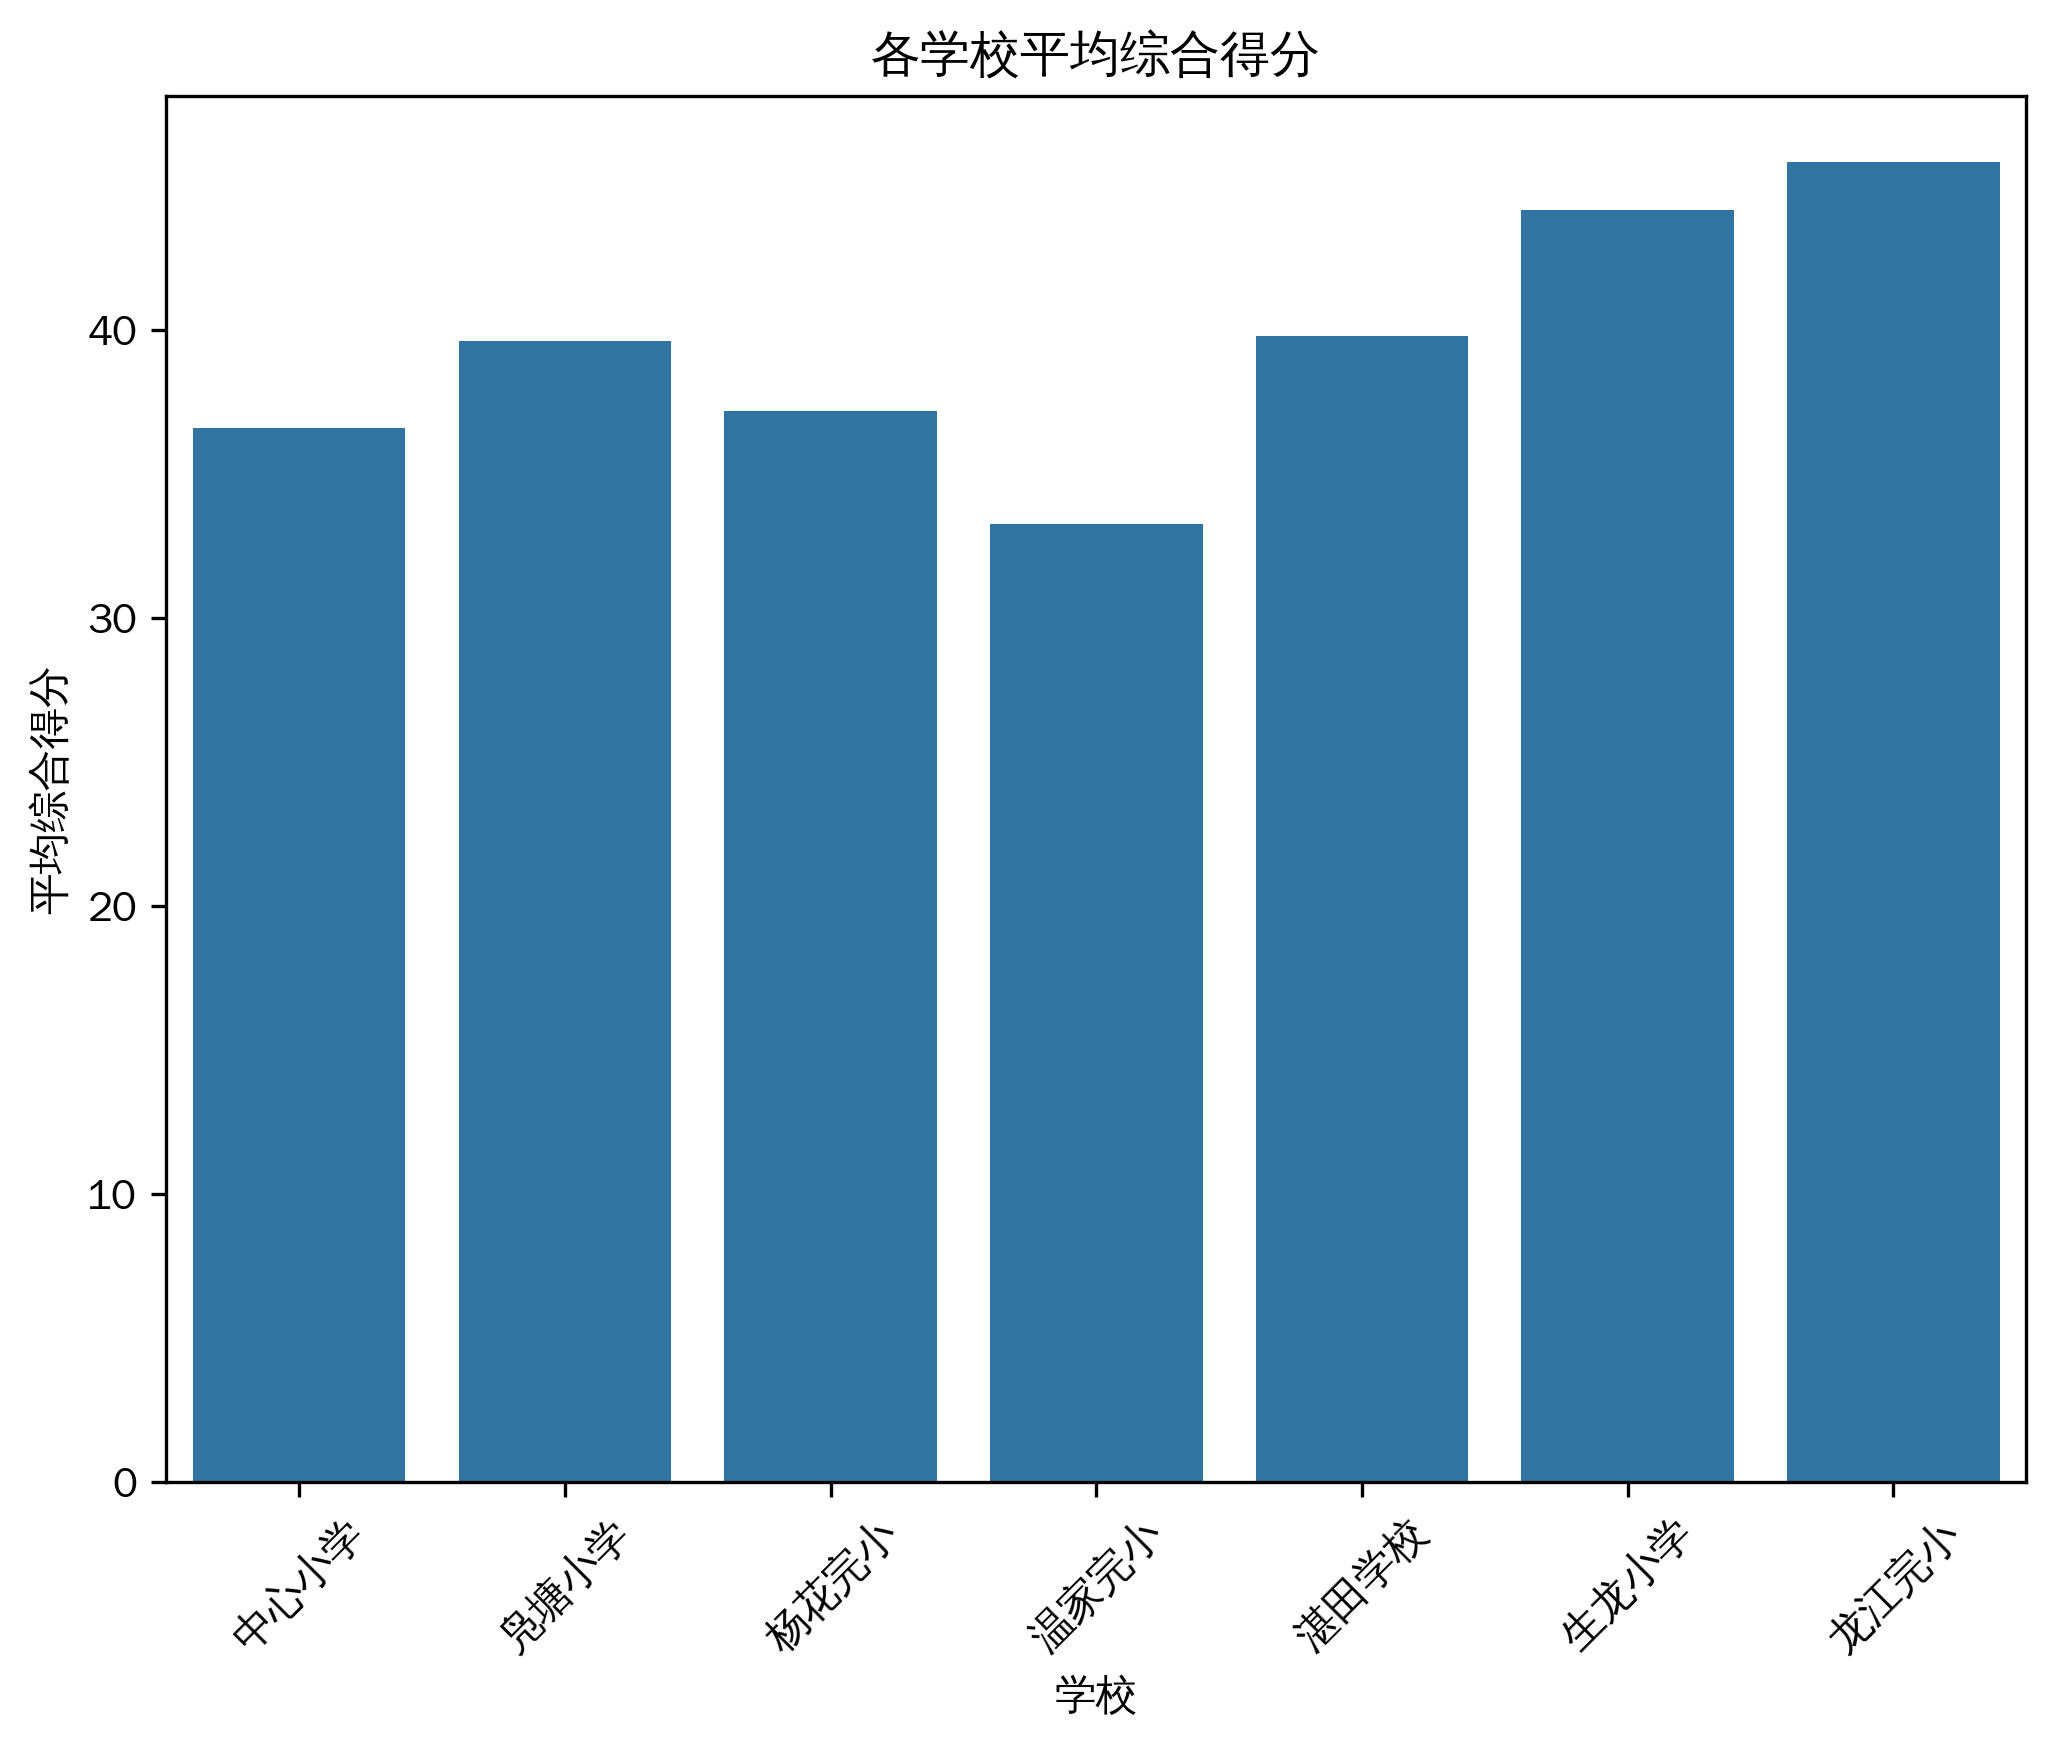
\includegraphics[width=0.6\textwidth]{fig/1.png}
    \caption{各学校平均综合得分}
\end{figure}

\begin{figure}[H]
    \centering
    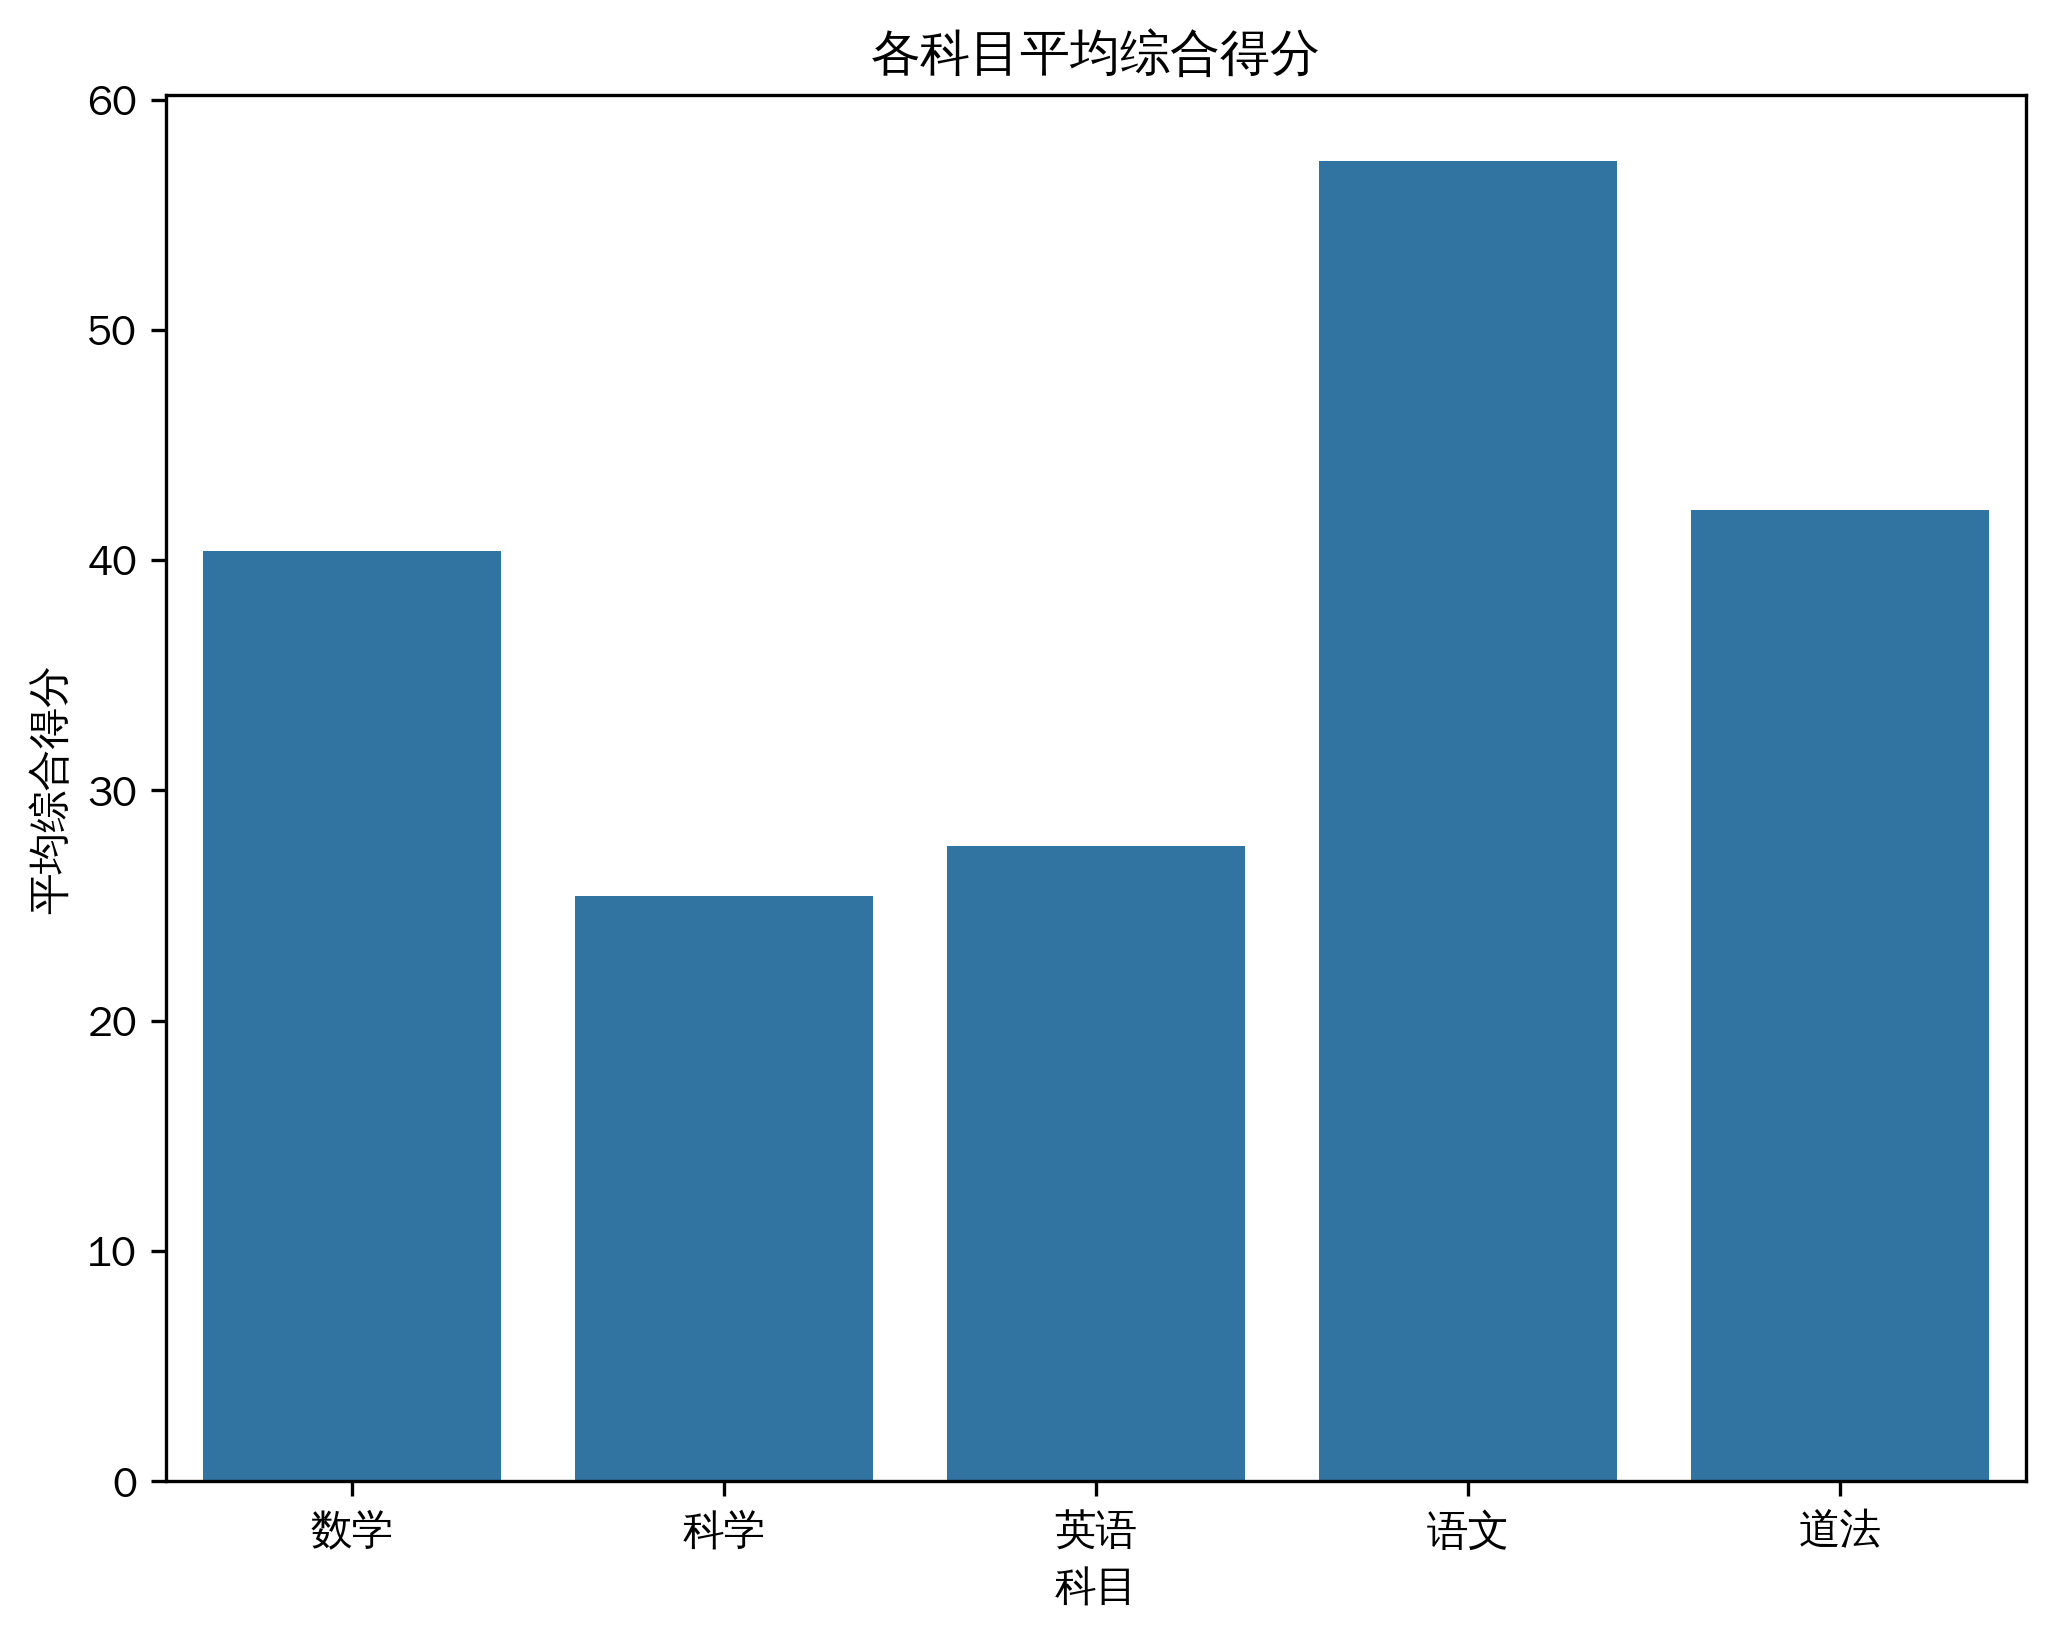
\includegraphics[width=0.7\textwidth]{fig/2.png}
    \caption{全镇各科目综合得分}
\end{figure}

\begin{figure}[H]
    \centering
    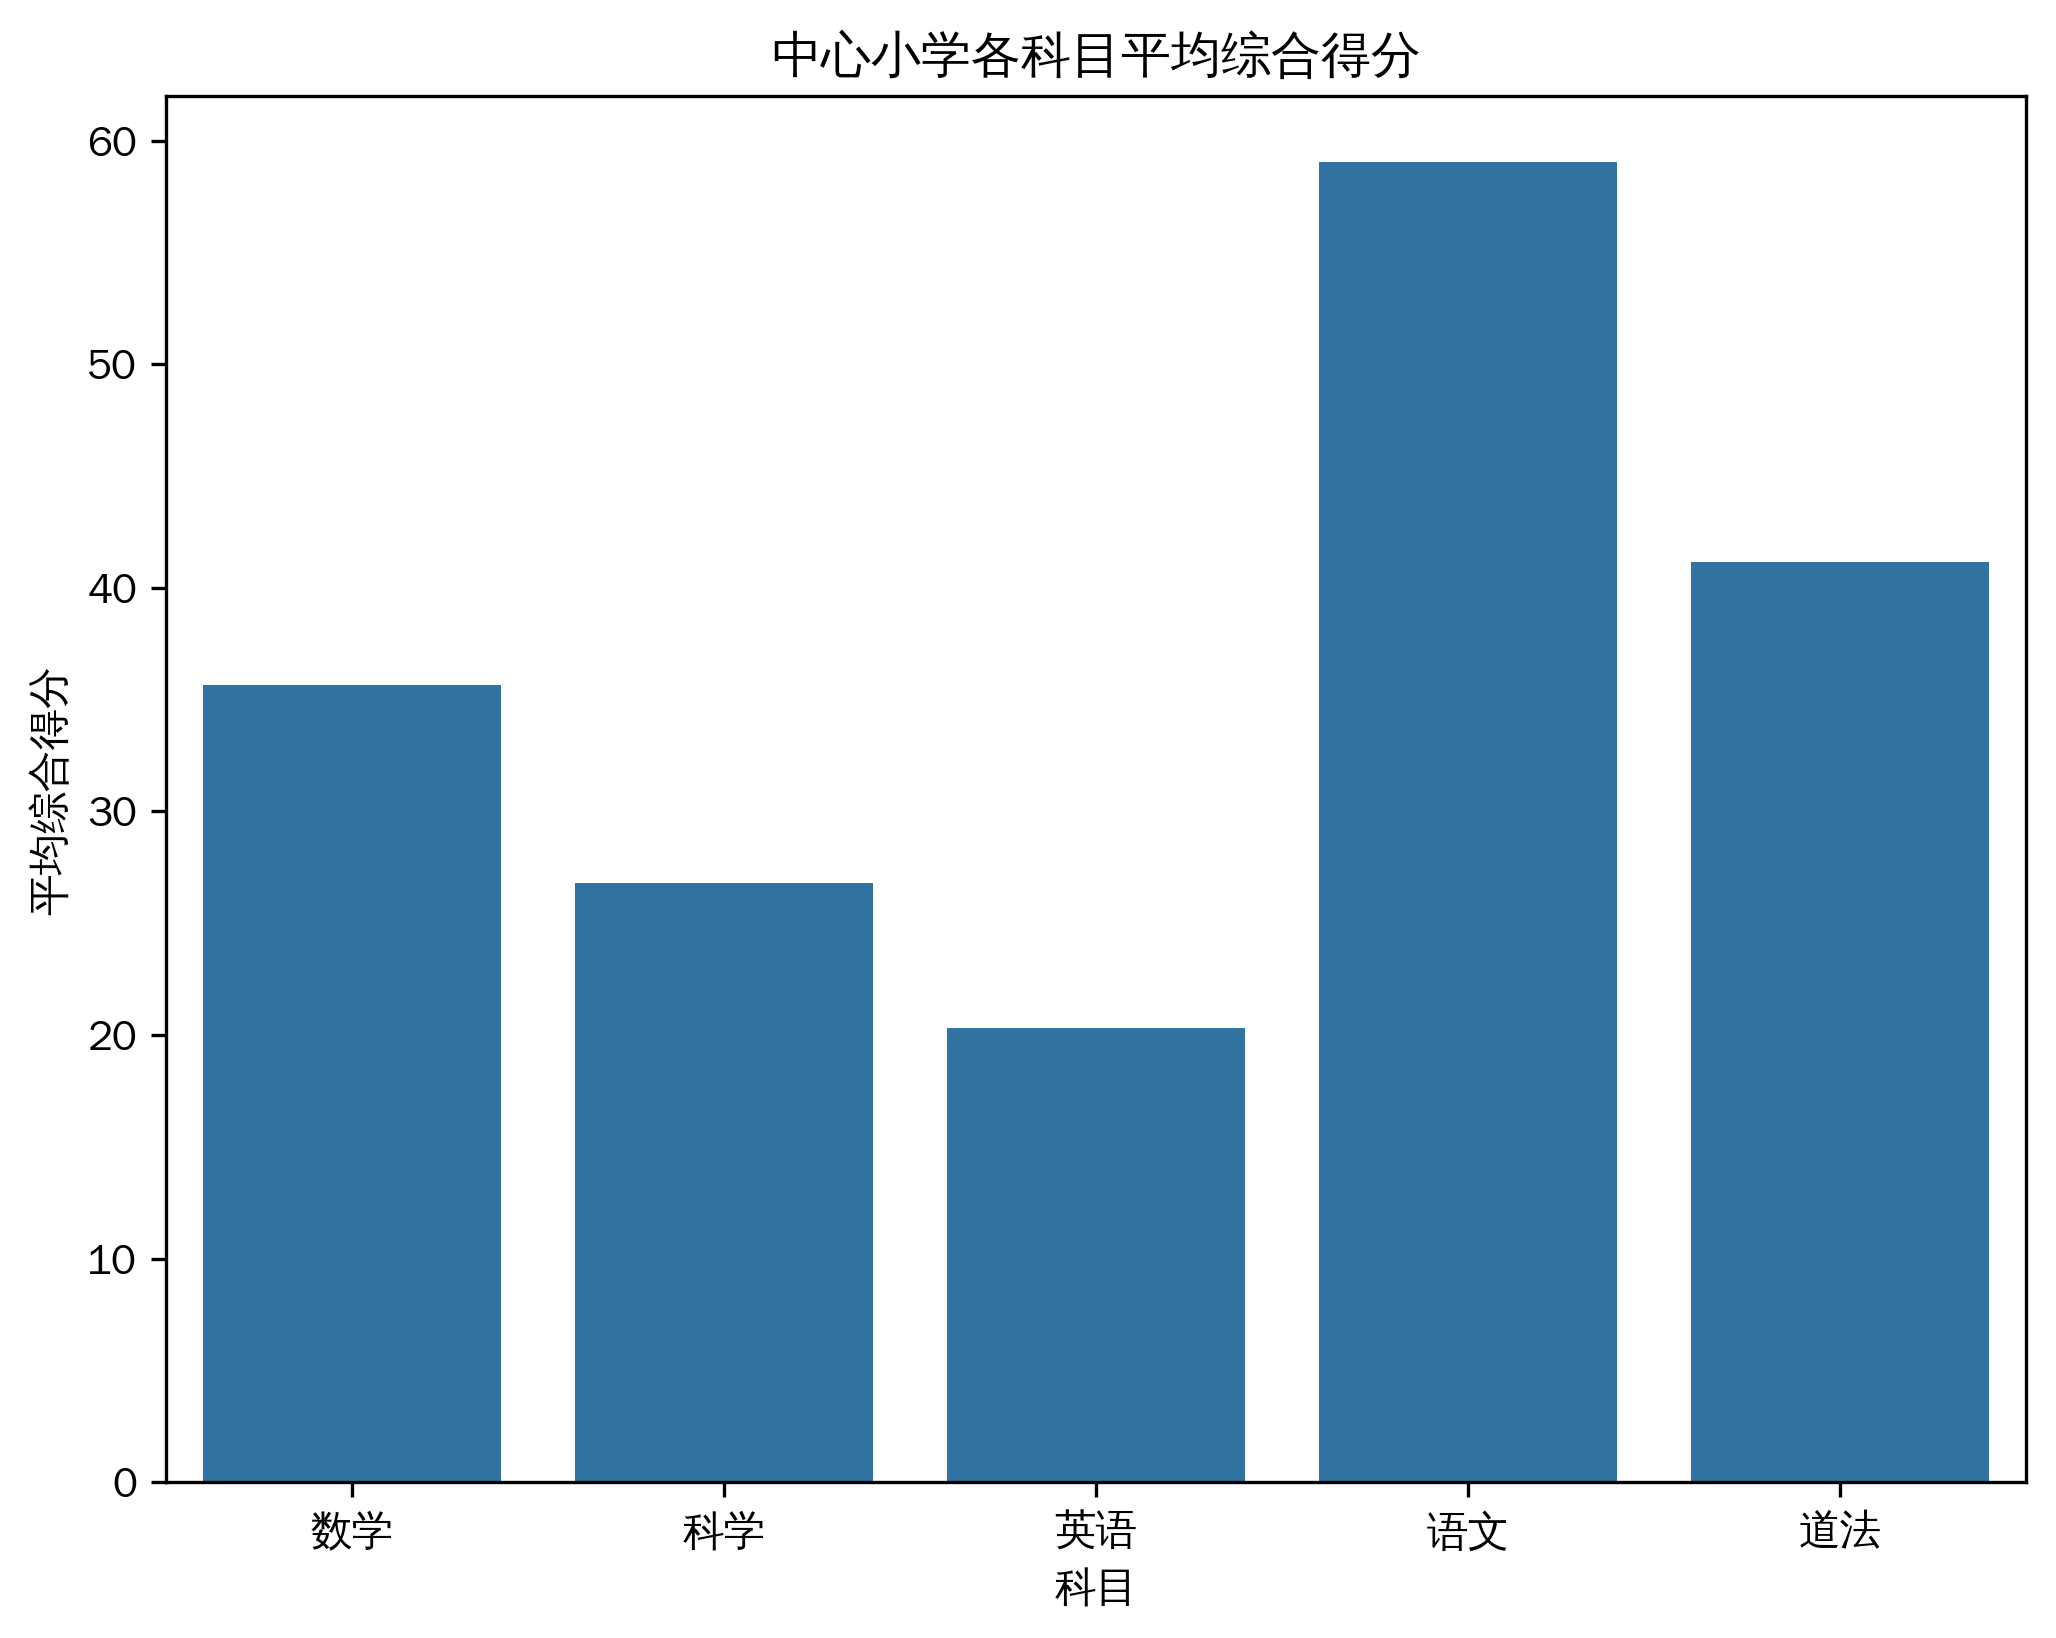
\includegraphics[width=0.7\textwidth]{fig/3.png}
    \caption{中心小学各科目综合得分}
\end{figure}

\begin{figure}[H]
    \centering
    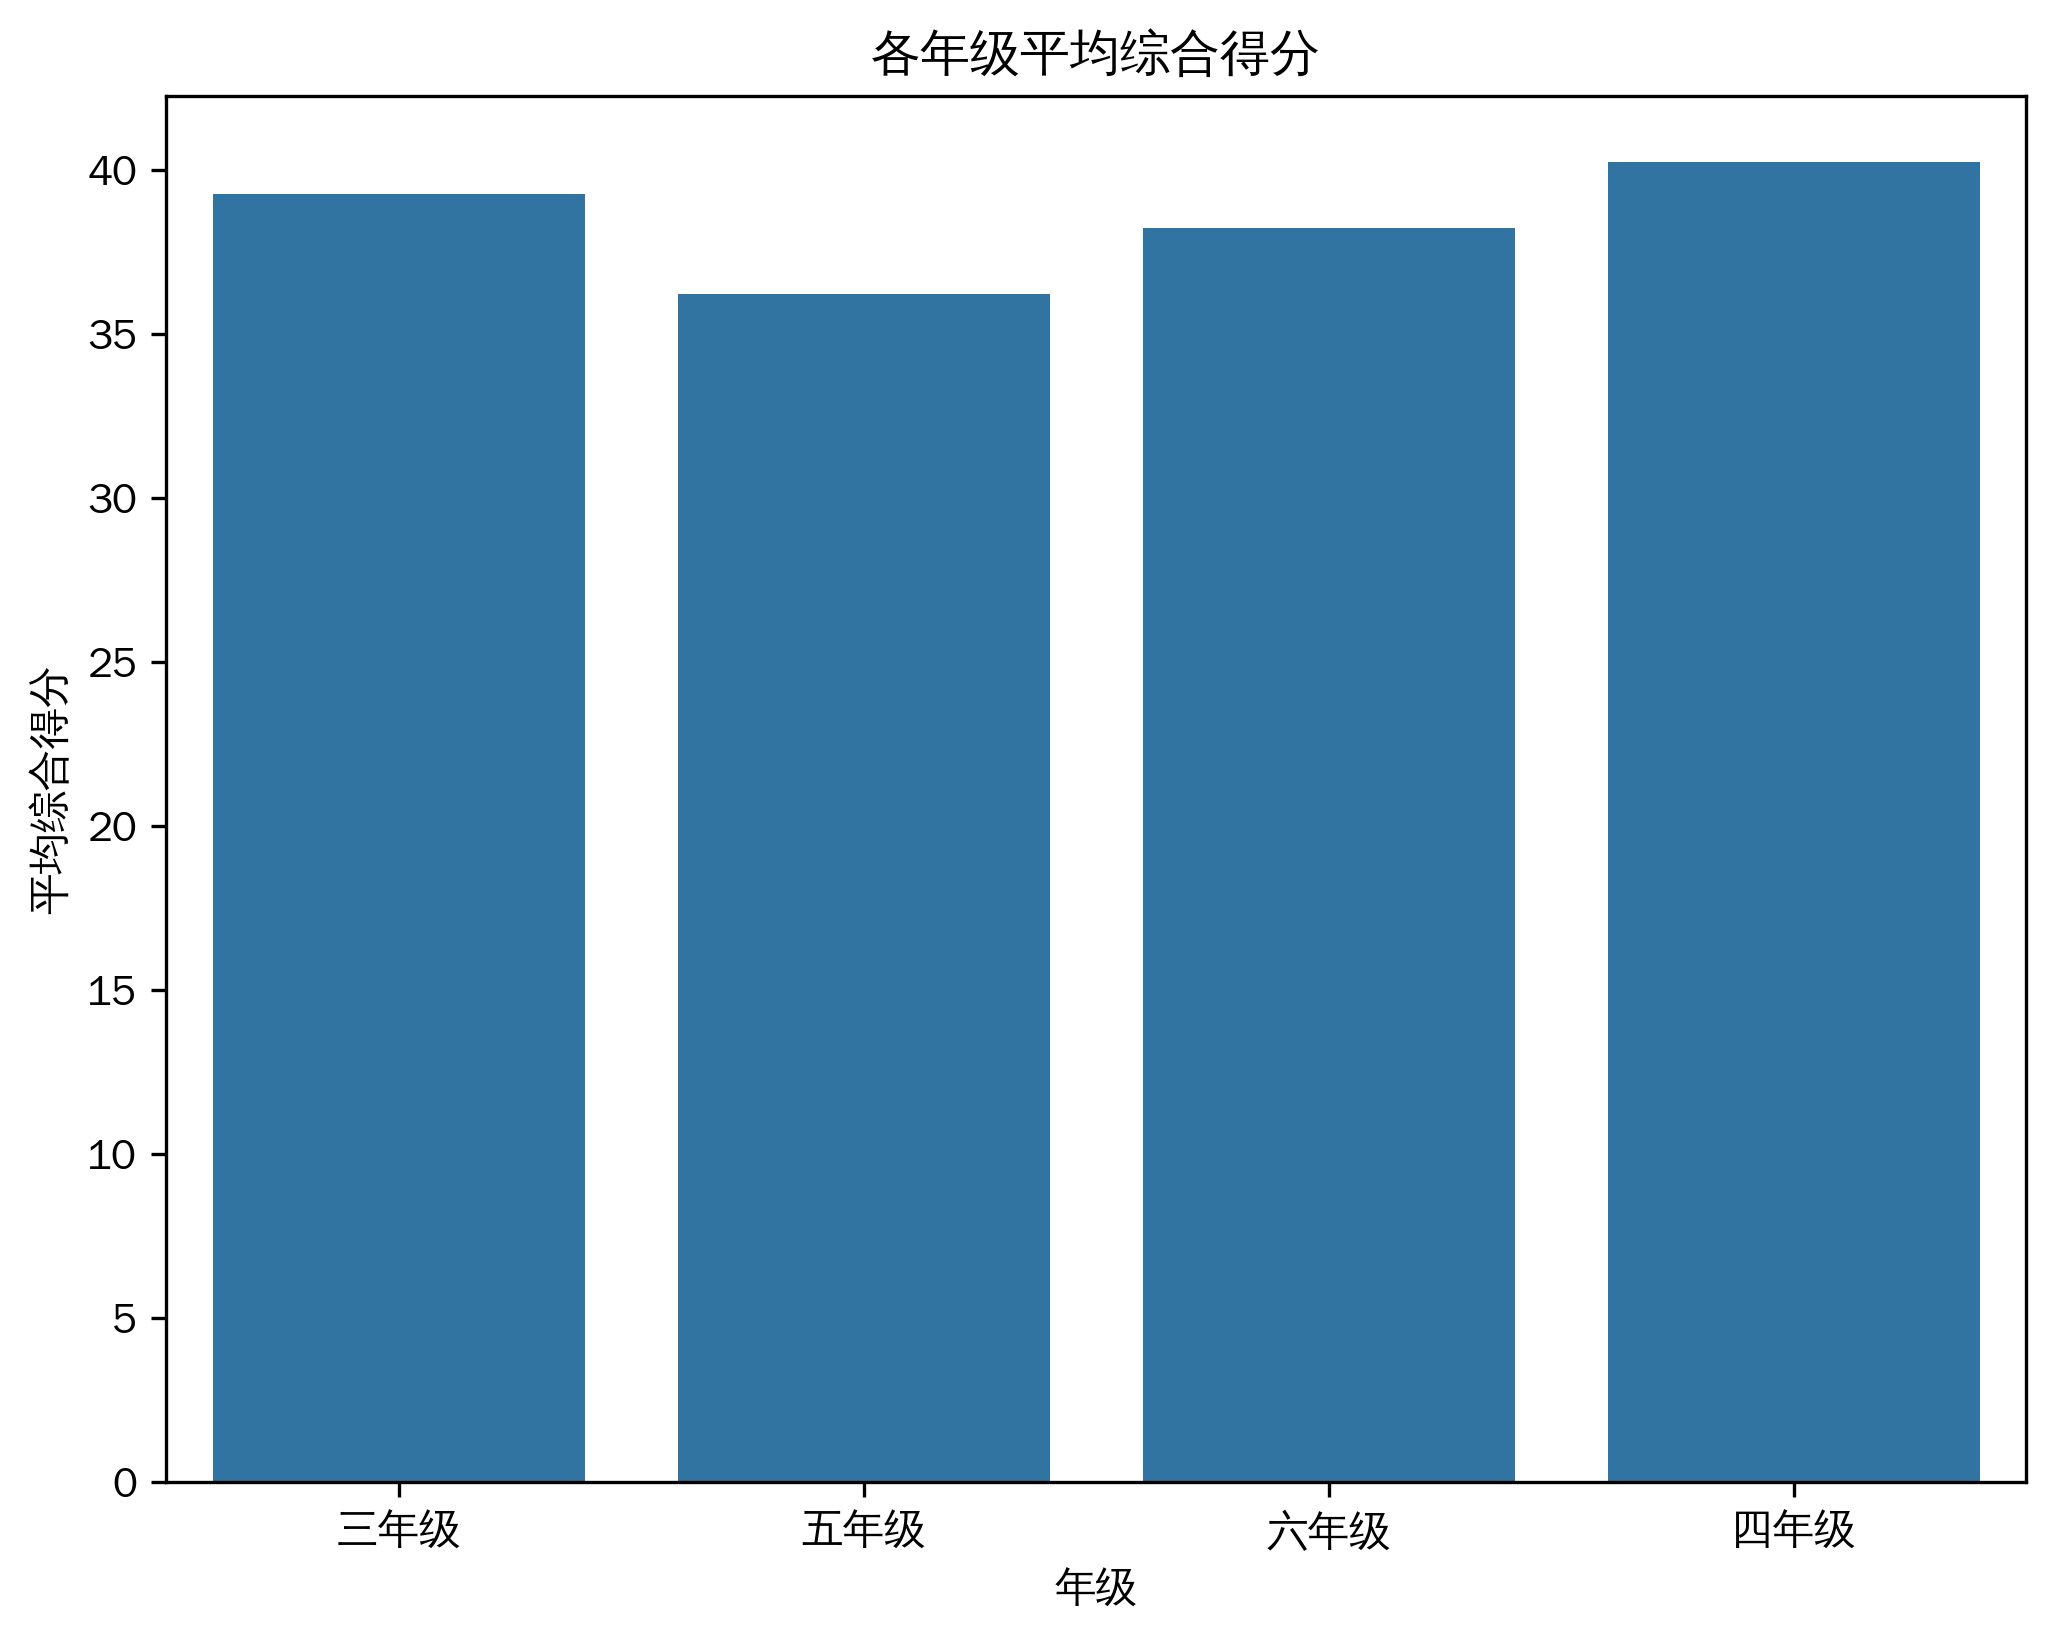
\includegraphics[width=0.7\textwidth]{fig/4.png}
    \caption{全镇各年级综合得分}
\end{figure}

\begin{figure}[H]
    \centering
    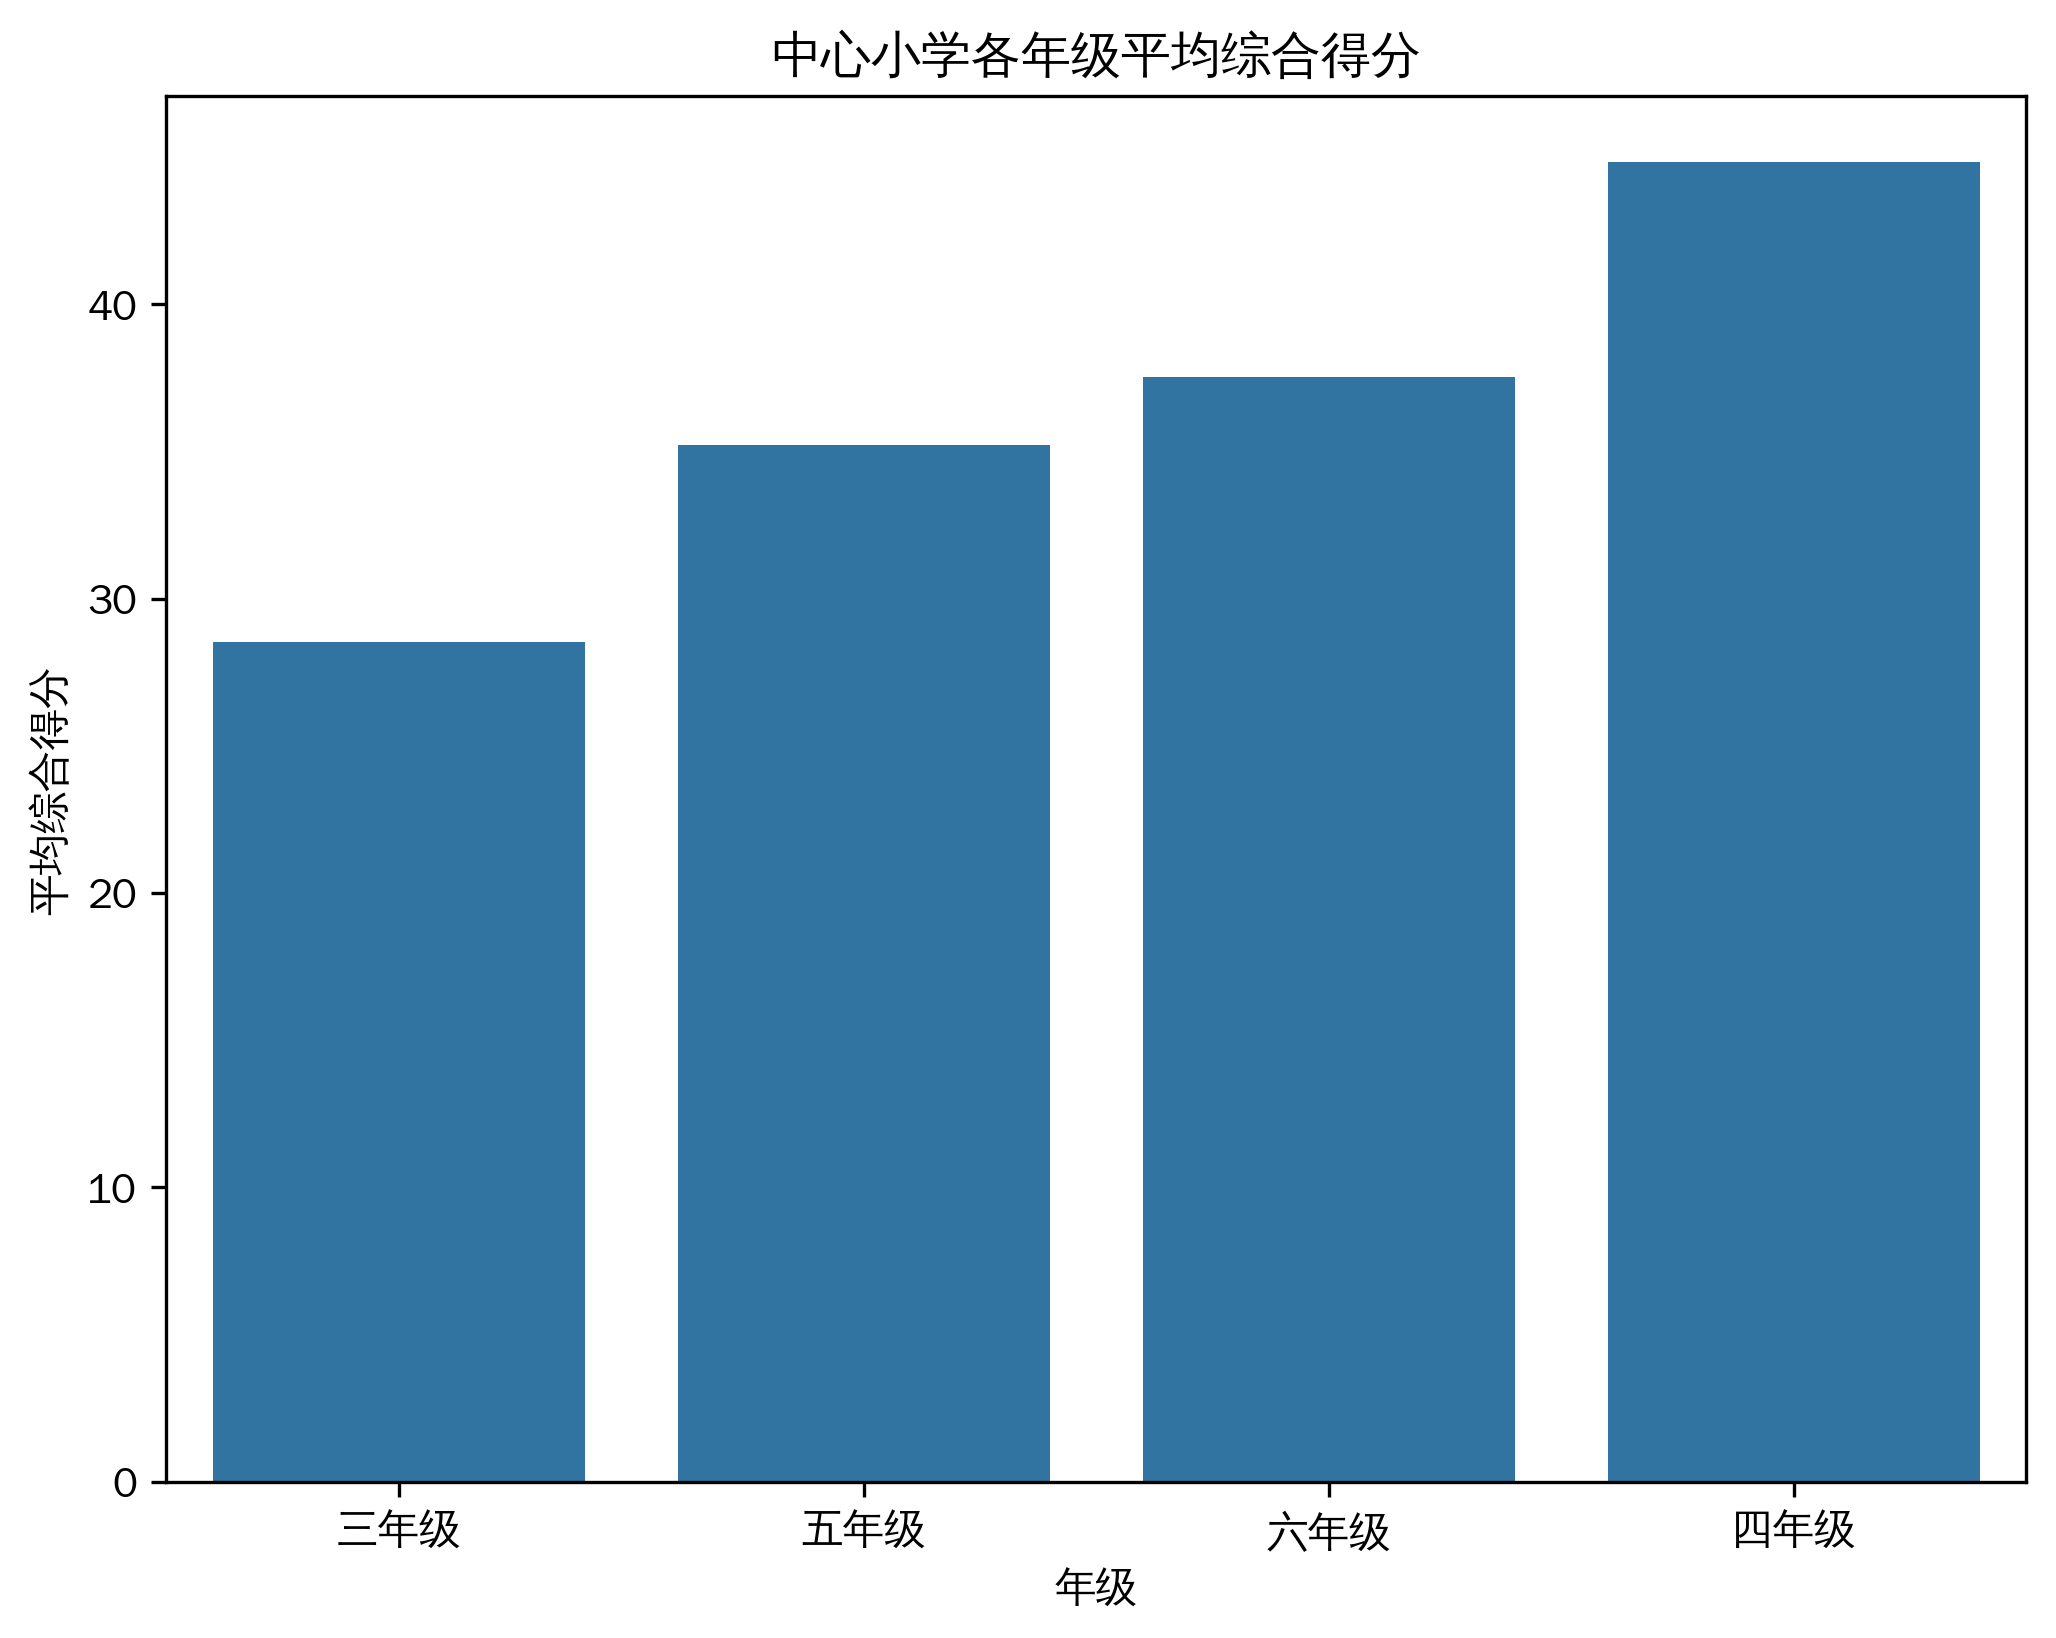
\includegraphics[width=0.7\textwidth]{fig/5.png}
    \caption{中心小学各年级综合得分}
\end{figure}

\begin{figure}[H]
    \centering
    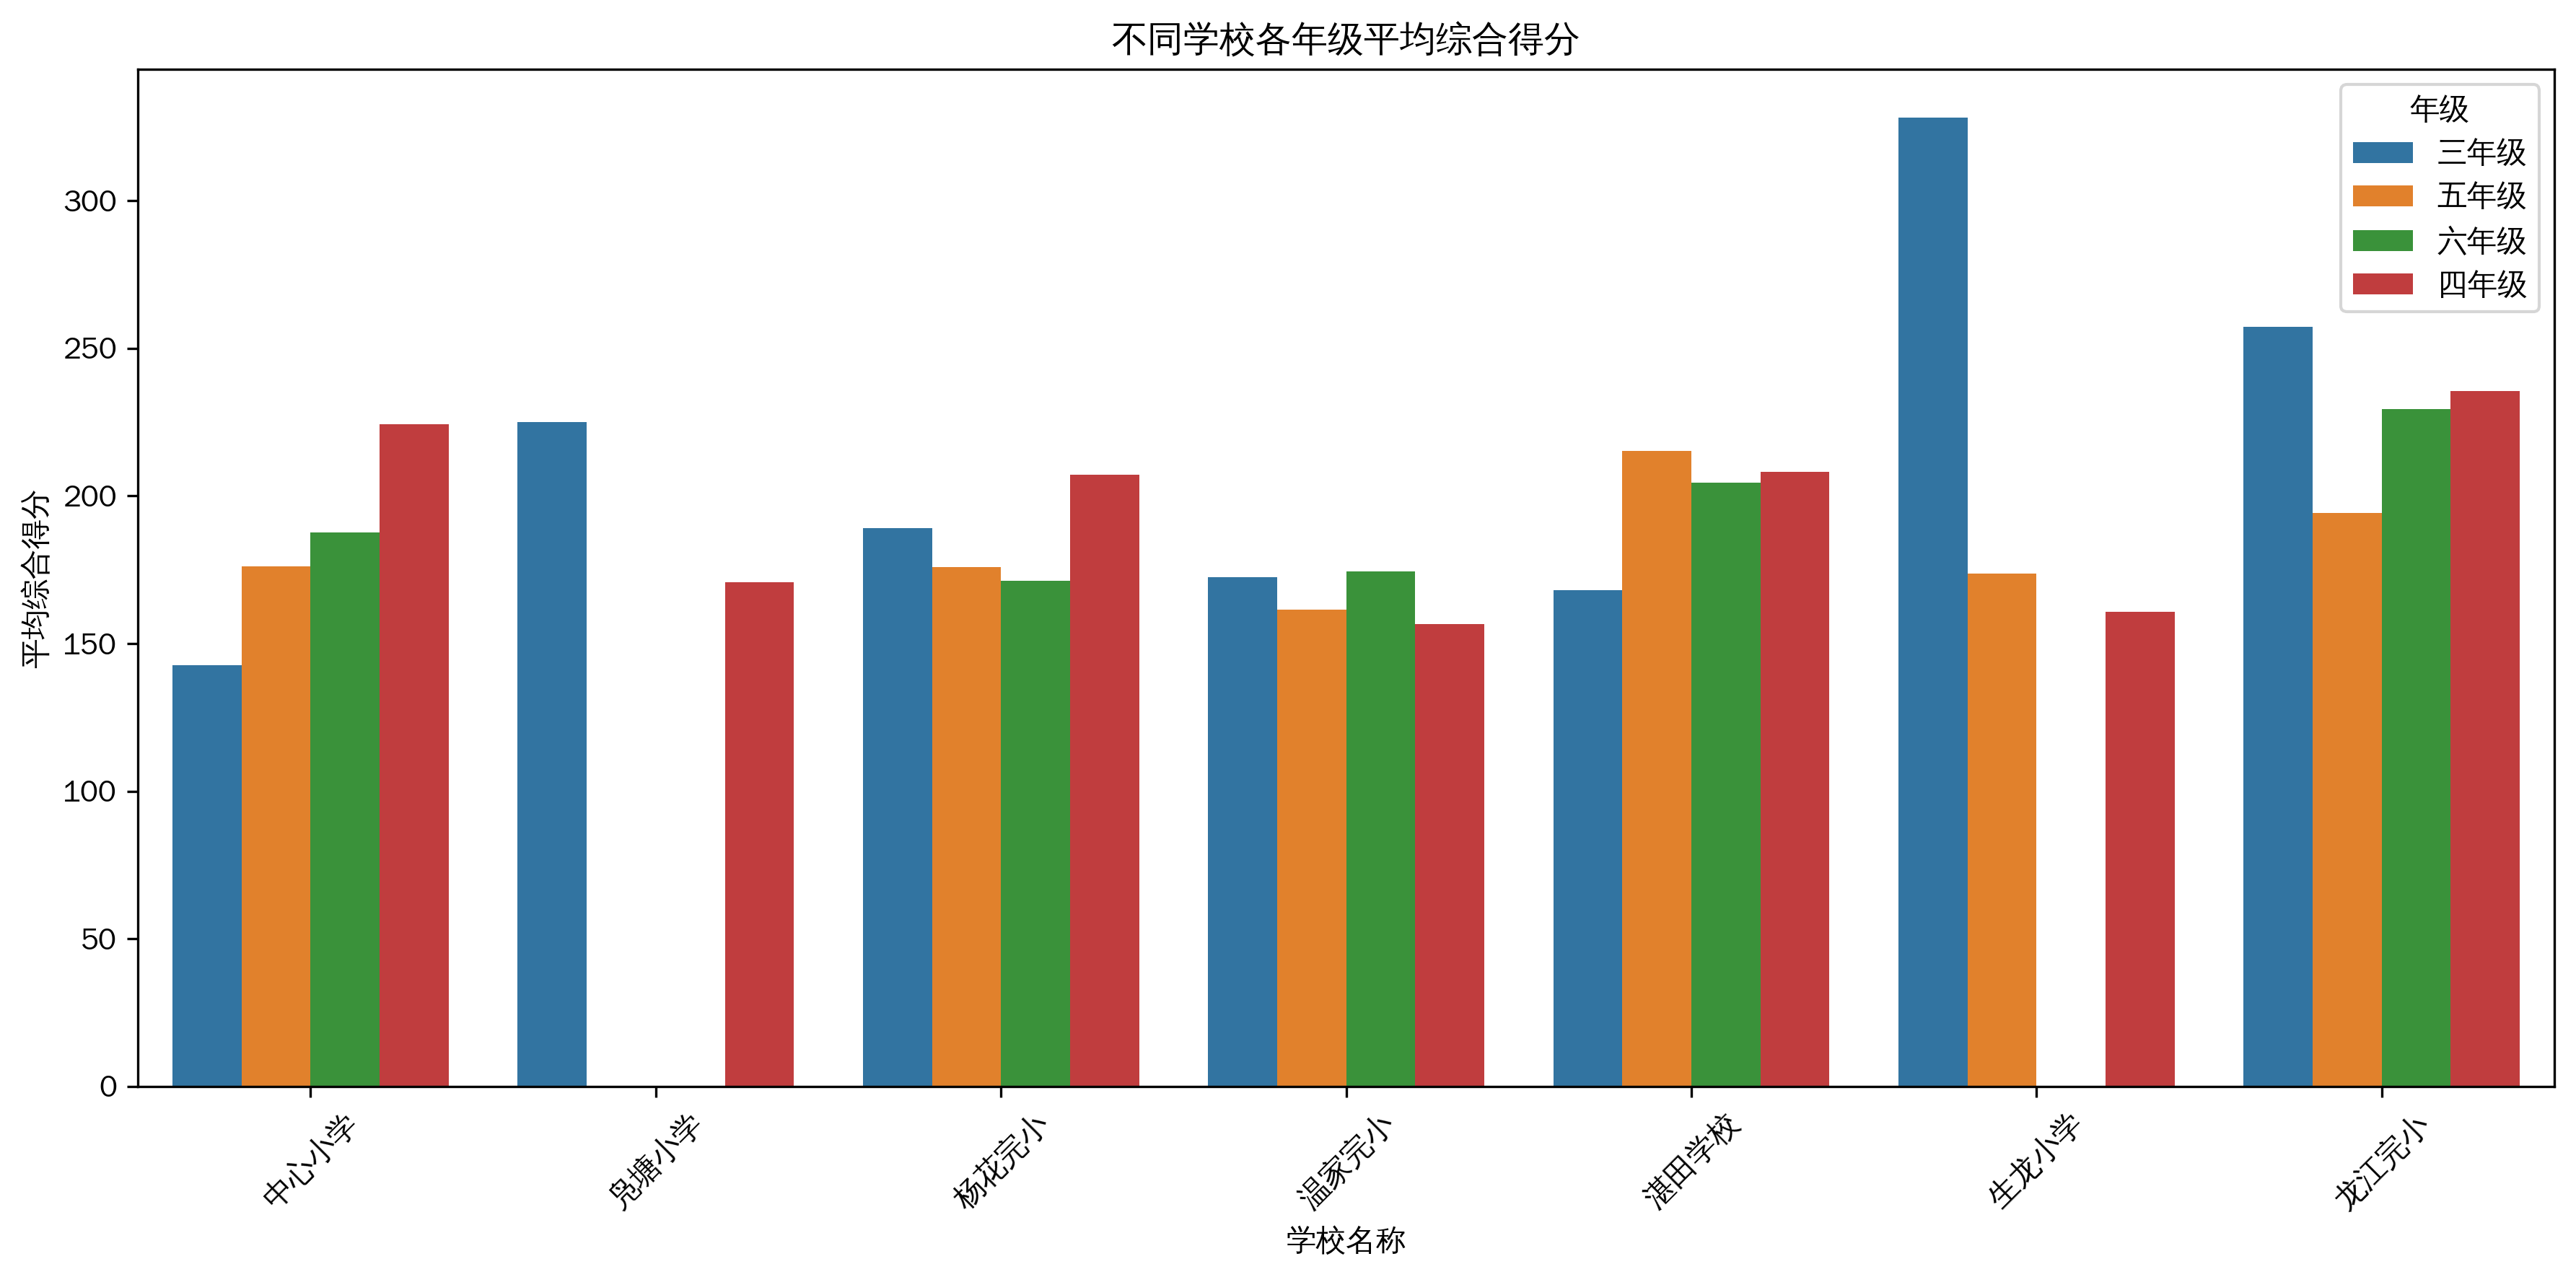
\includegraphics[width=1\textwidth]{fig/6.png}
    \caption{各学校各年级平均综合得分}
\end{figure}

\begin{figure}[H]
    \centering
    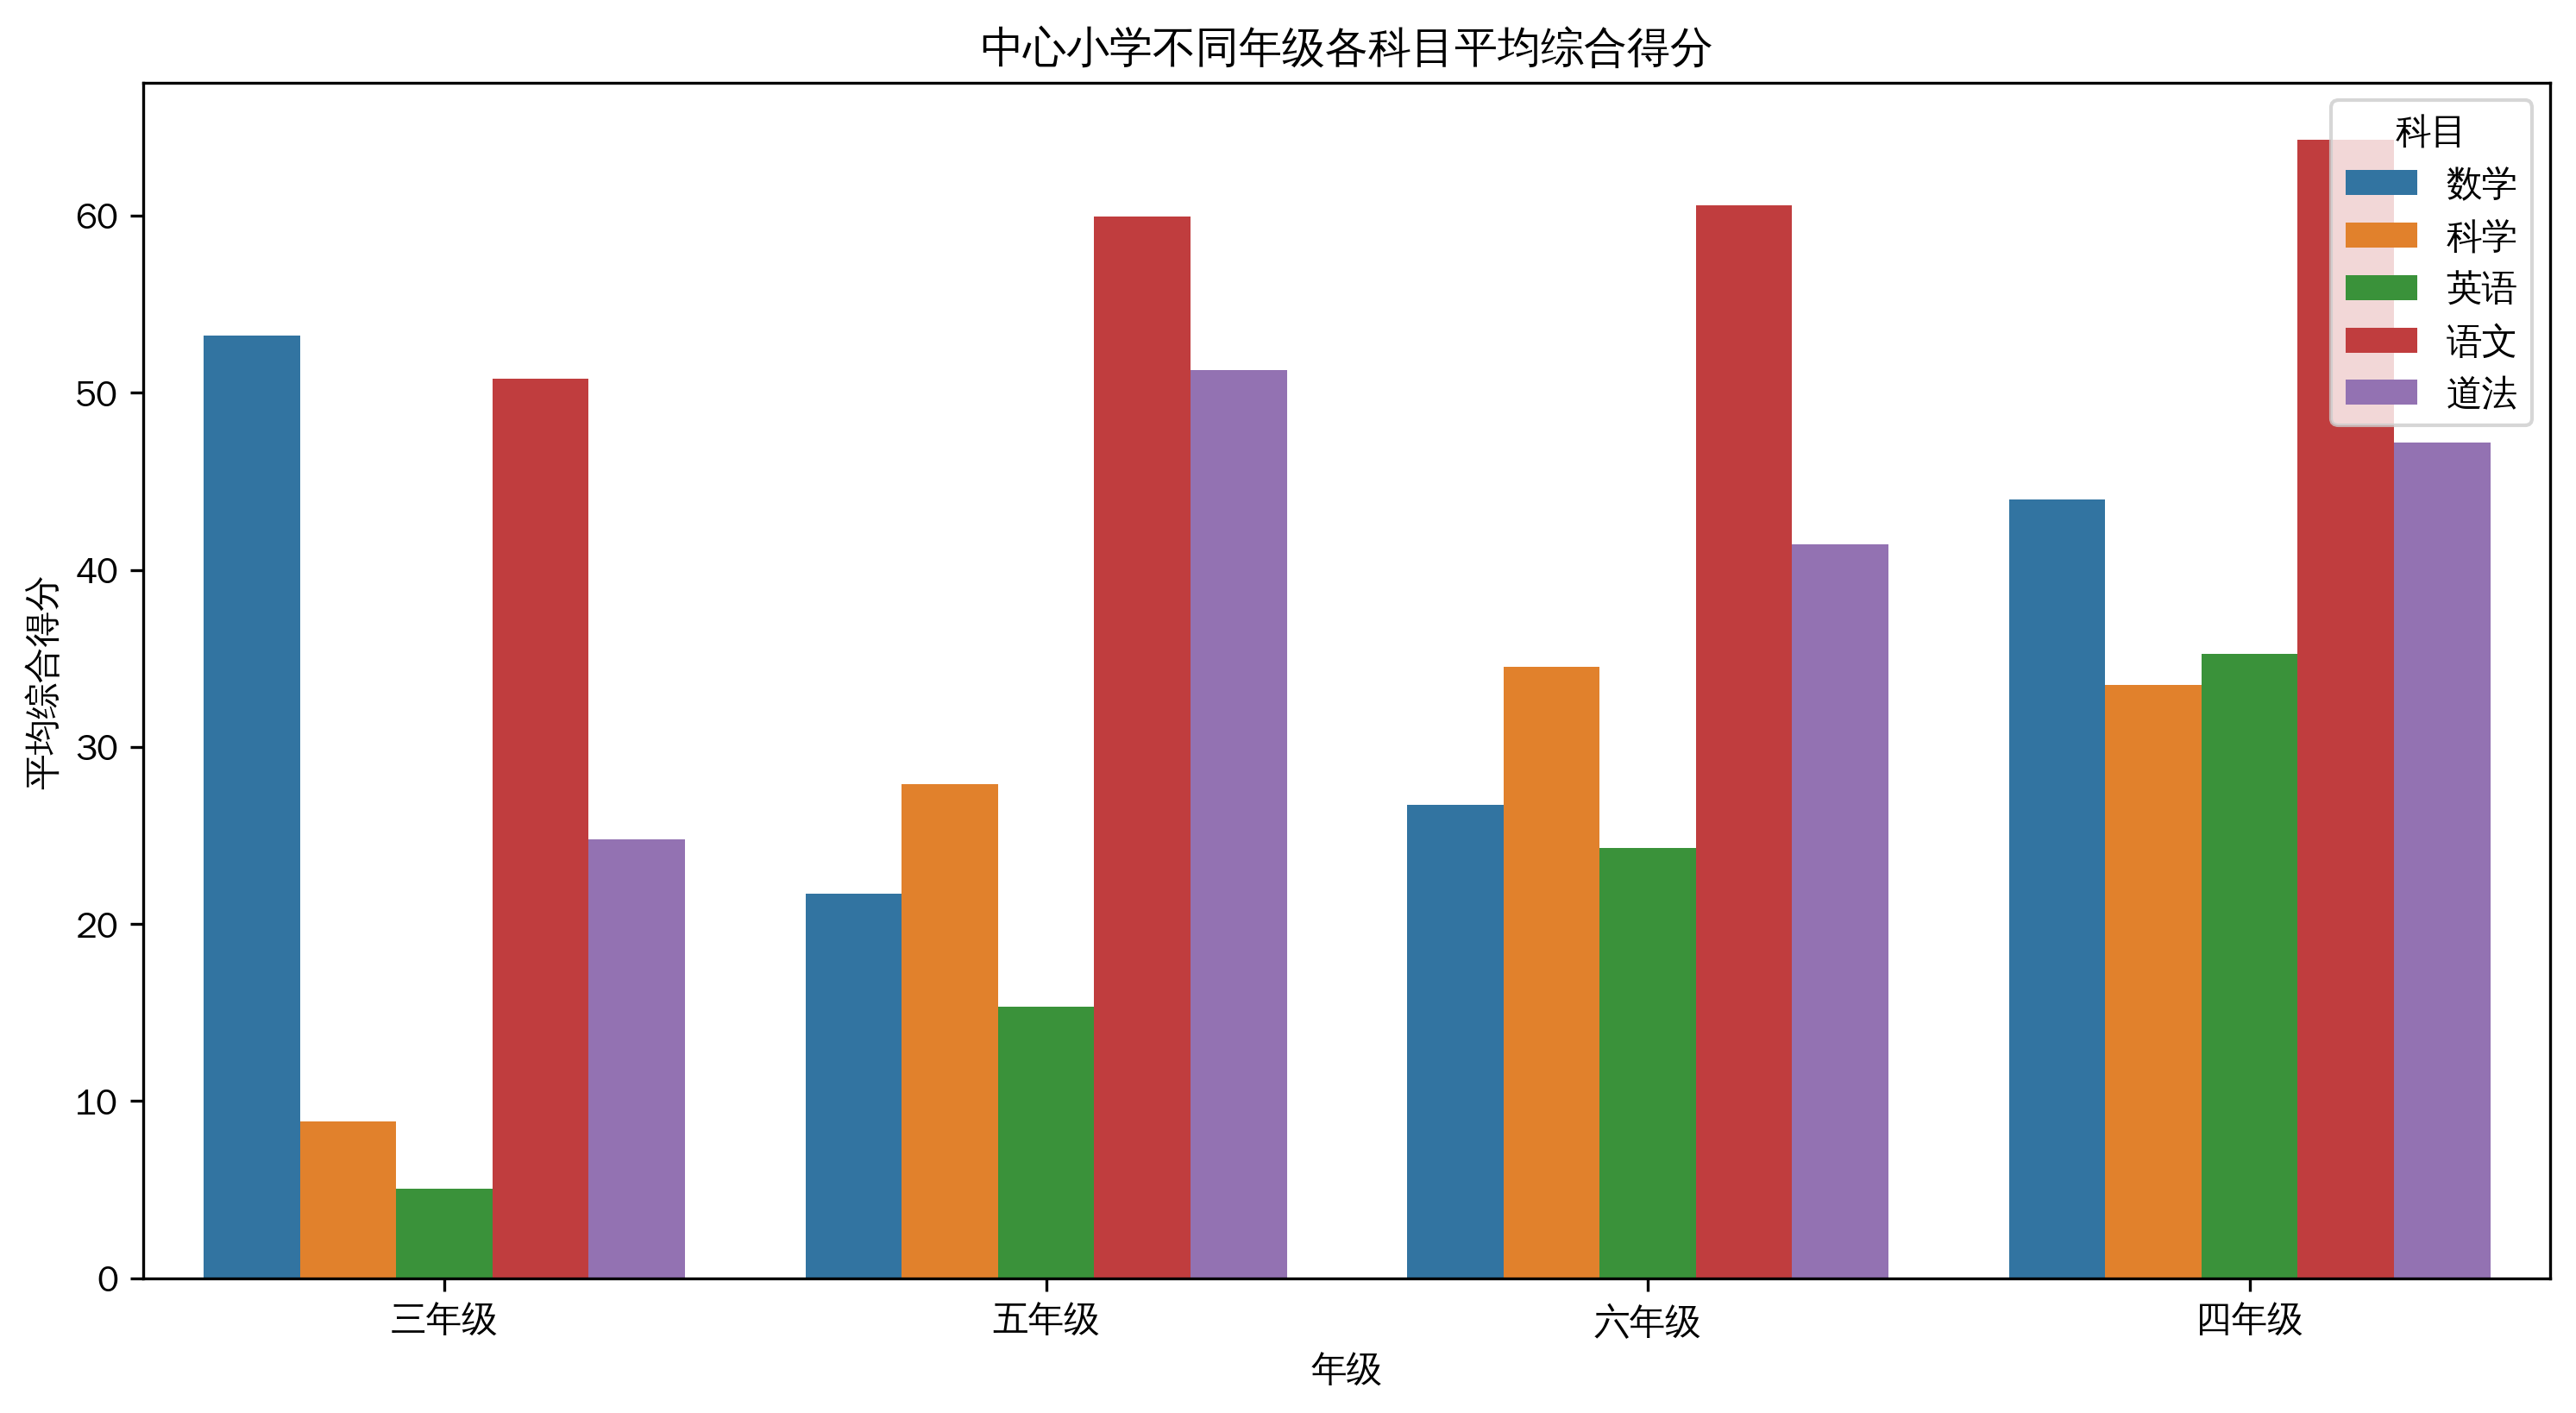
\includegraphics[width=1\textwidth]{fig/7.png}
    \caption{中心小学各年级平均综合得分}
\end{figure}

\begin{figure}[H]
    \centering
    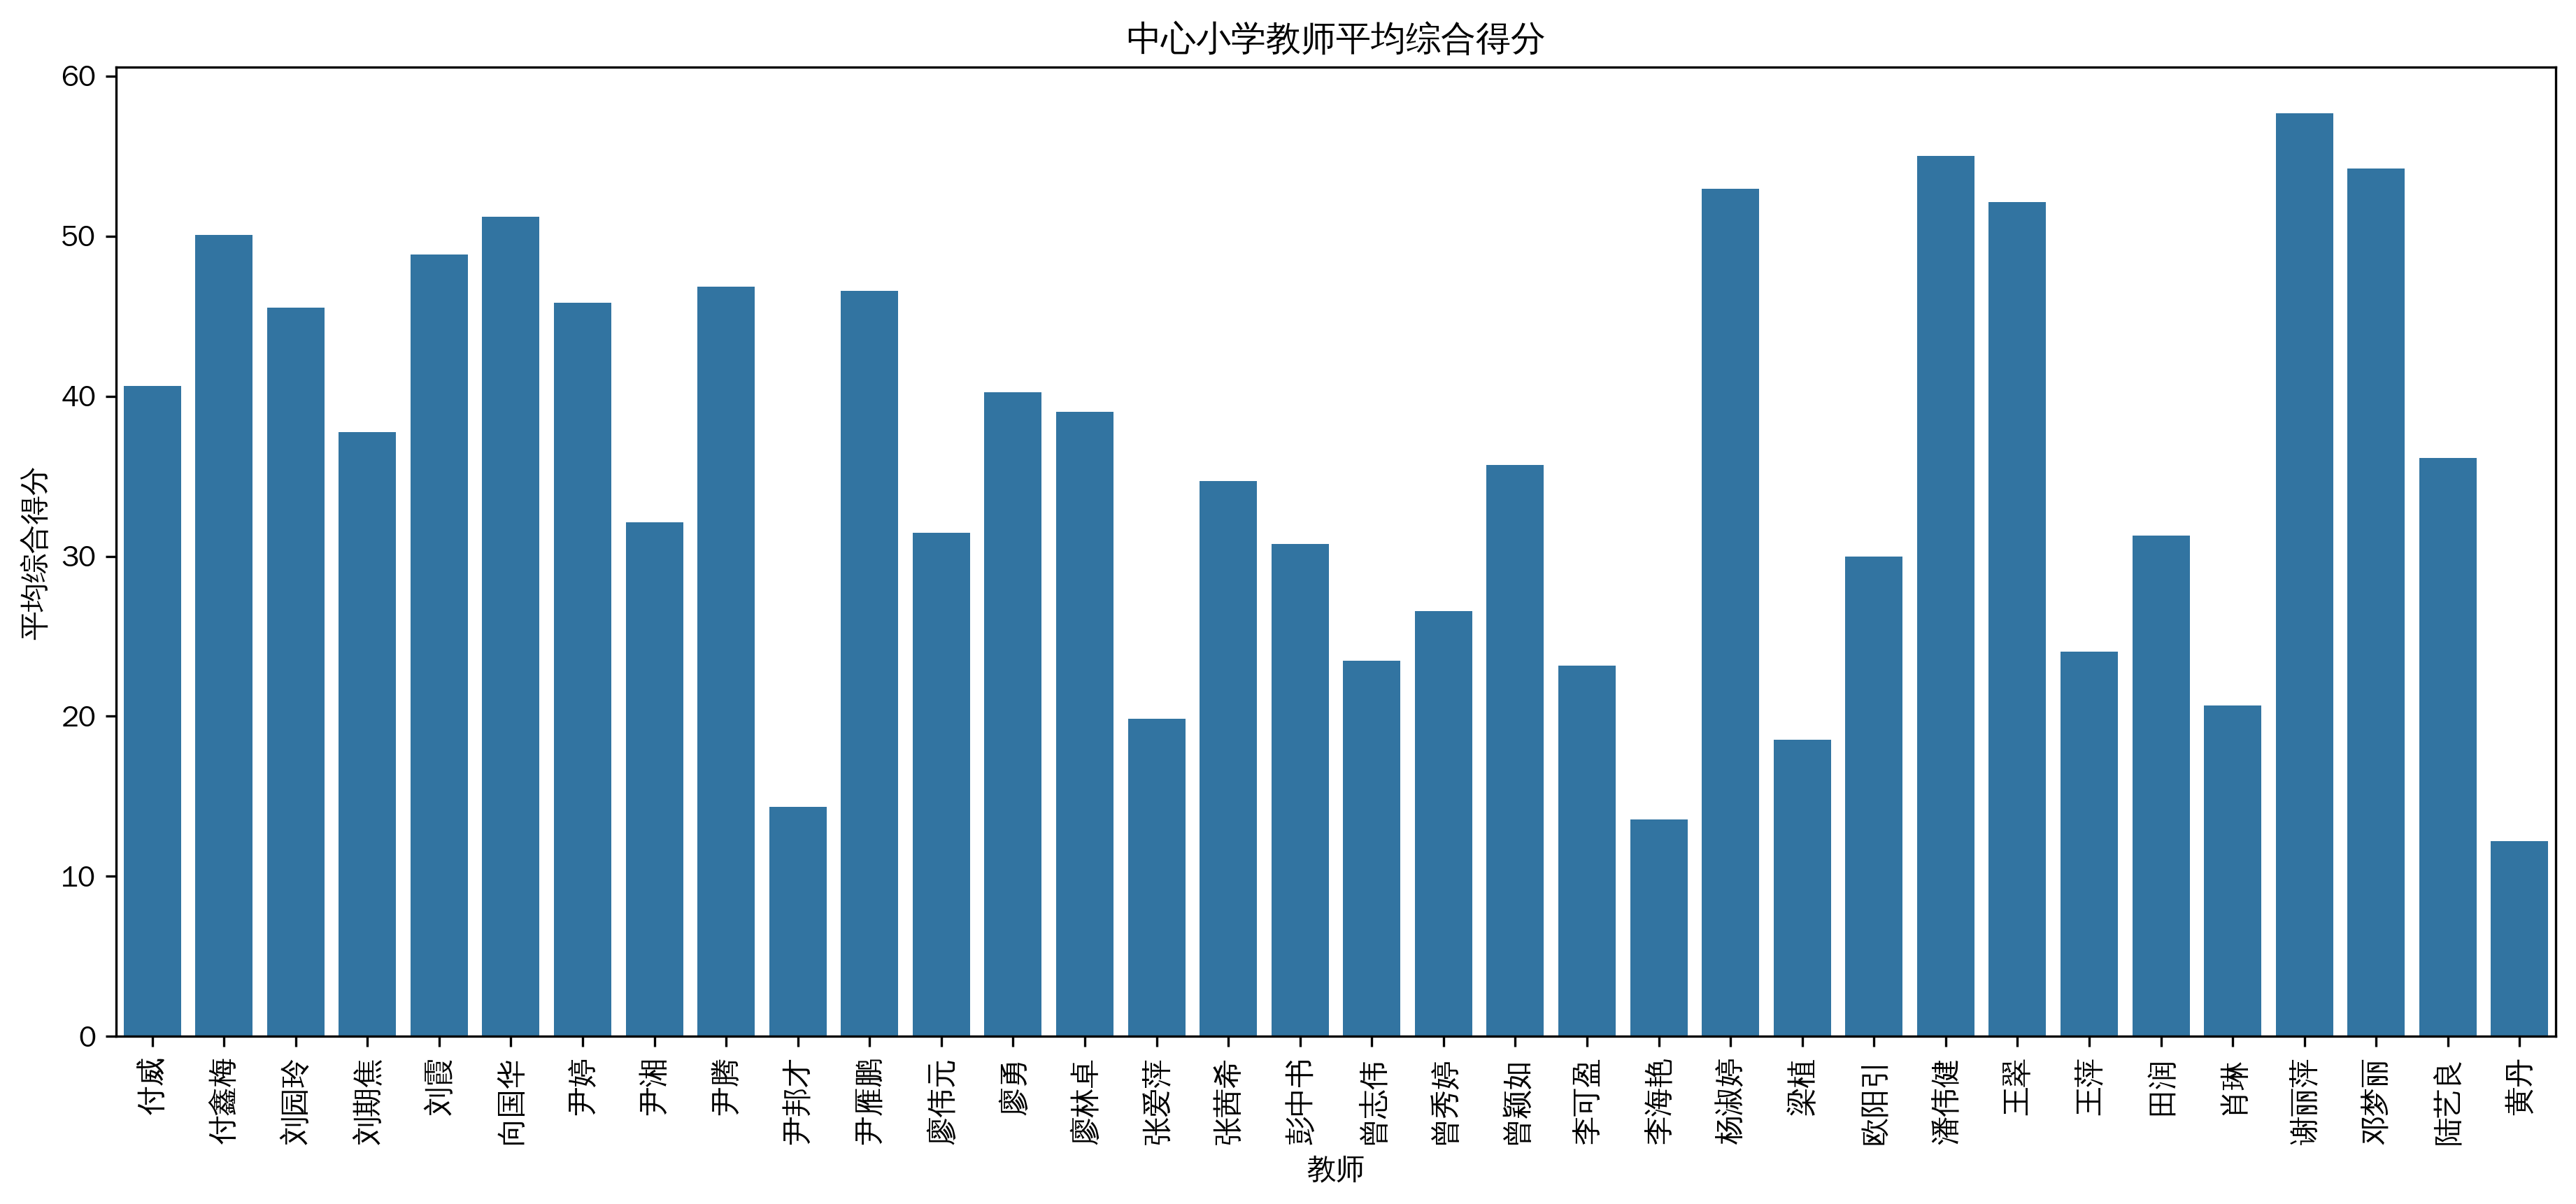
\includegraphics[width=1\textwidth]{fig/8.png}
    \caption{中心小学教师平均综合得分}
\end{figure}

\begin{figure}[H]
    \centering
    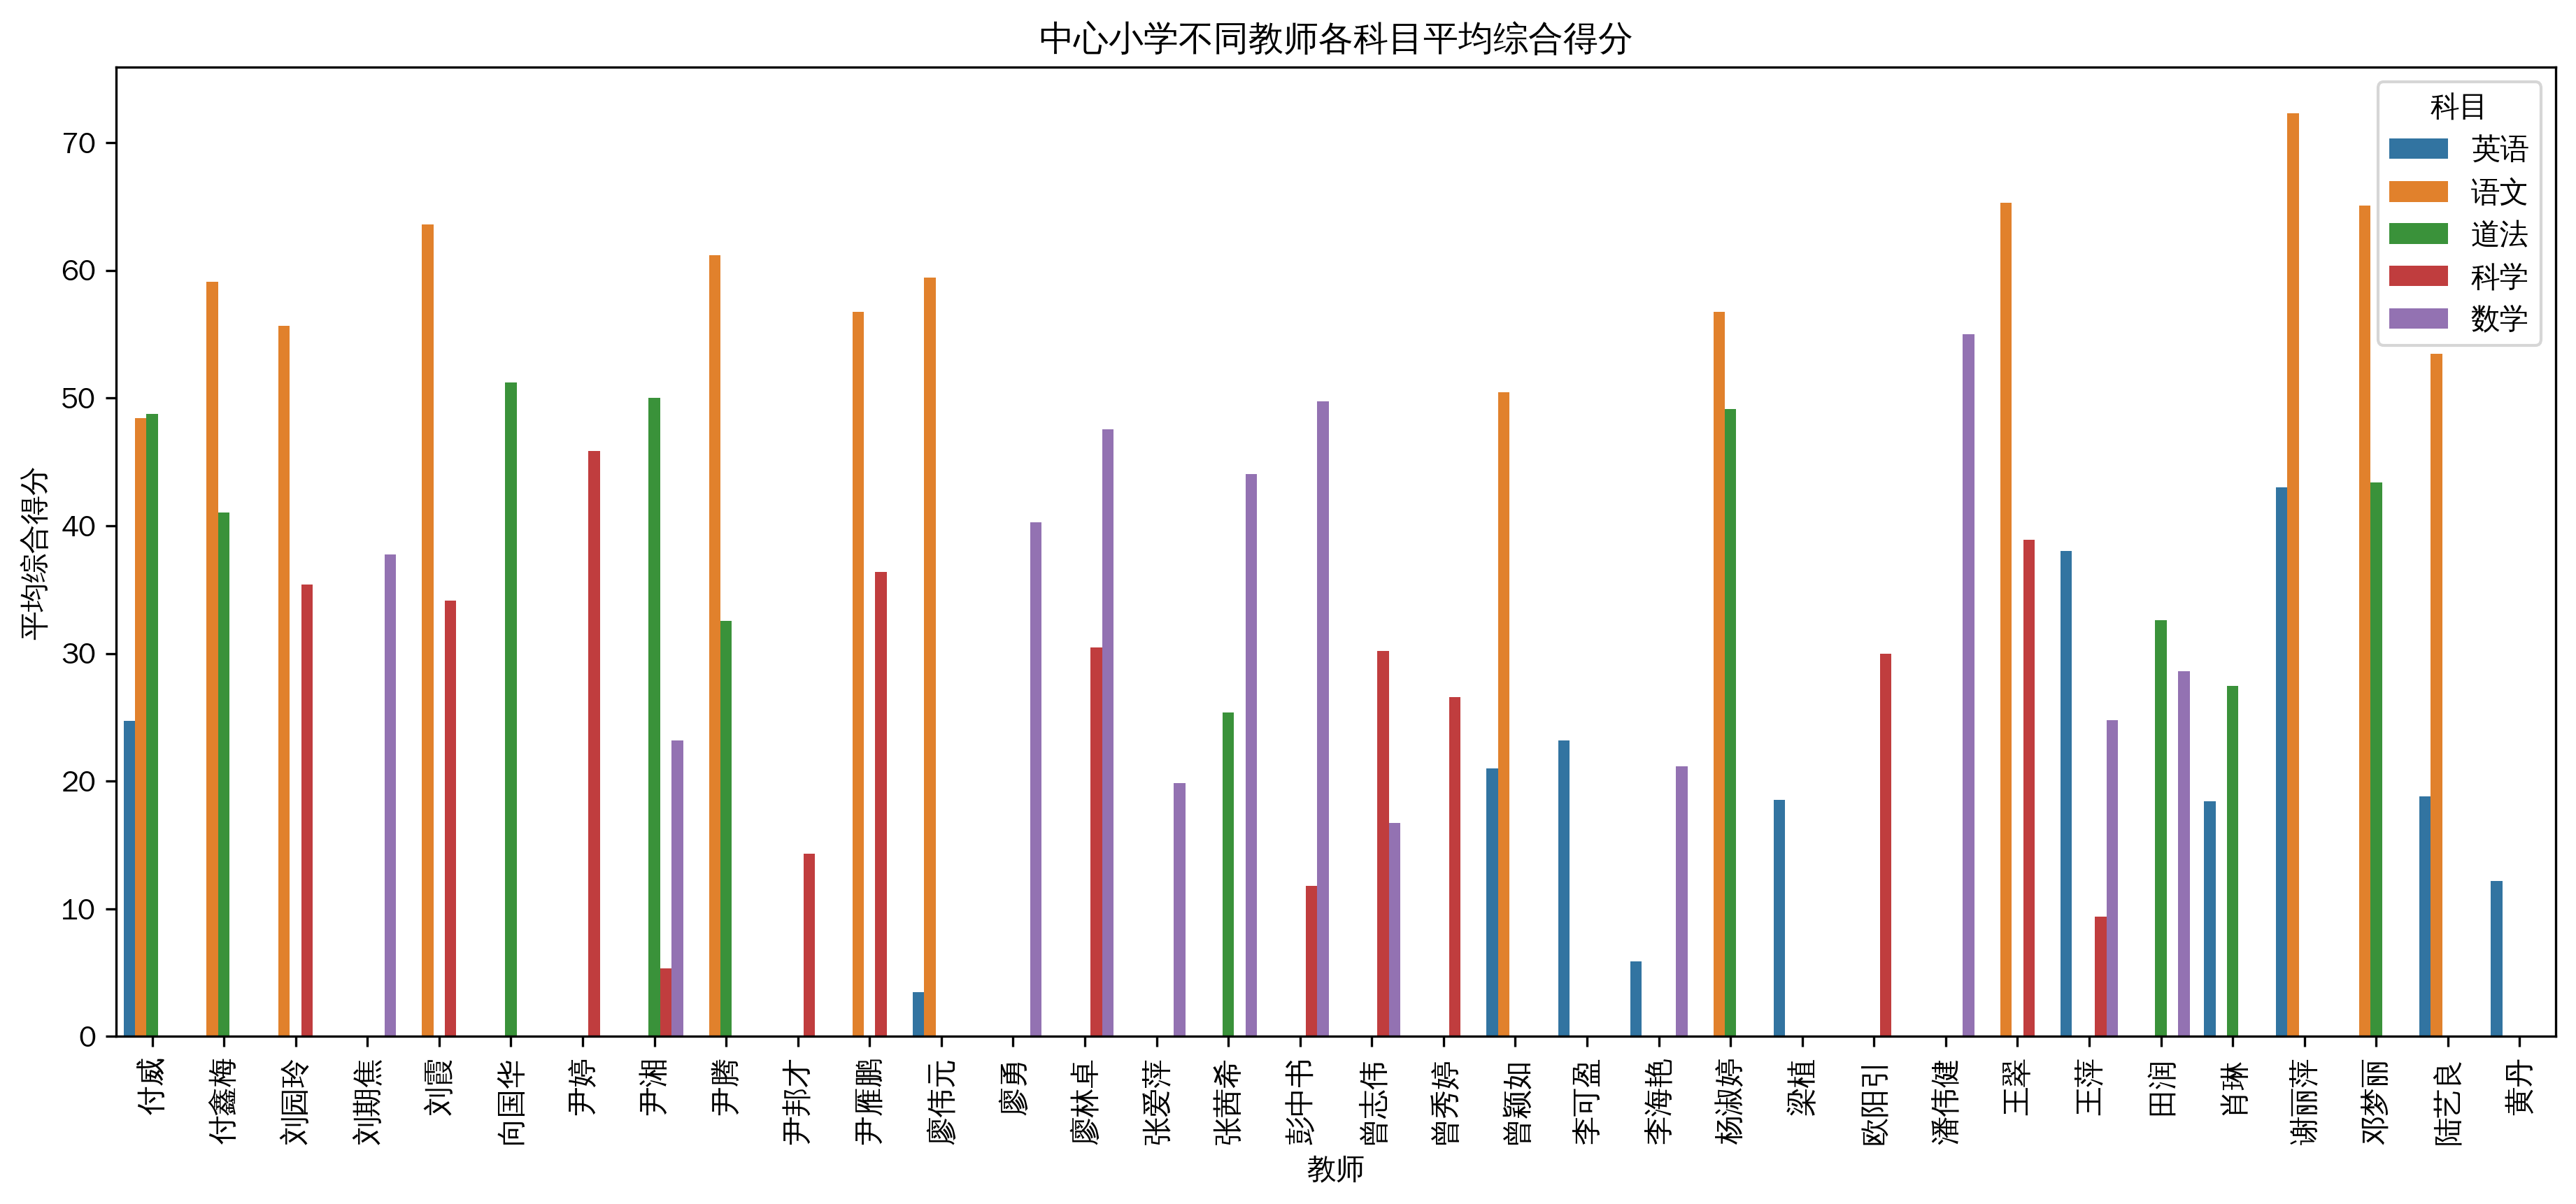
\includegraphics[width=1\textwidth]{fig/9.png}
    \caption{中心小学教师各科目平均综合得分}
\end{figure}

% ...如有更多图片,继续按文件名顺序插入...

% 添加参考文献
% \bibliographystyle{plain}
% \bibliography{references}

\end{document}
